%% Beispiel-Präsentation mit LaTeX Beamer im KIT-Design
%% entsprechend den Gestaltungsrichtlinien vom 1. August 2020
%%
%% Siehe https://sdqweb.ipd.kit.edu/wiki/Dokumentvorlagen

%% Beispiel-Präsentation
\documentclass[en]{sdqbeamer} 
 
%% Titelbild
\titleimage{../images/title_header_4}

%% Gruppenlogo
\grouplogo{teco_logo.png} 

%% Gruppenname und Breite (Standard: 50 mm)
\groupname{
Chair of Pervasive Computing Systems/TECO\\
Institute of Telematics, Department of Informatics\\
}
%\groupnamewidth{50mm}

% Beginn der Präsentation

\title[Ear-Based Temperature Probing]{Ear-Based Temperature Probing: \\ Sensor Placement and Fusion for Wearable Applications}
\subtitle{Chair of Pervasive Computing Systems / TECO} 
\author[David Laubenstein]{David Laubenstein, Supervisor: Tobias Röddiger}

\date[05/10/2023]{May 10, 2023}

% Literatur 
 
\usepackage[bibstyle=numeric,hyperref,backend=biber]{biblatex}
\usepackage[inkscapeformat=png]{svg}
\addbibresource{../thesis-doc/Literature.bib}
\bibhang1em

\begin{document}
 
%Titelseite
\KITtitleframe

%Inhaltsverzeichnis
% sollte weg laut betreuern
% \begin{frame}{Inhaltsverzeichnis}
% \tableofcontents
% \end{frame}

\section{Motivation}
\begin{frame}{Motivation}
    \begin{itemize}
        \item current state of temperature measurement \cite{TemperatureDigitalGlassa}
    \end{itemize}
    \begin{center}
        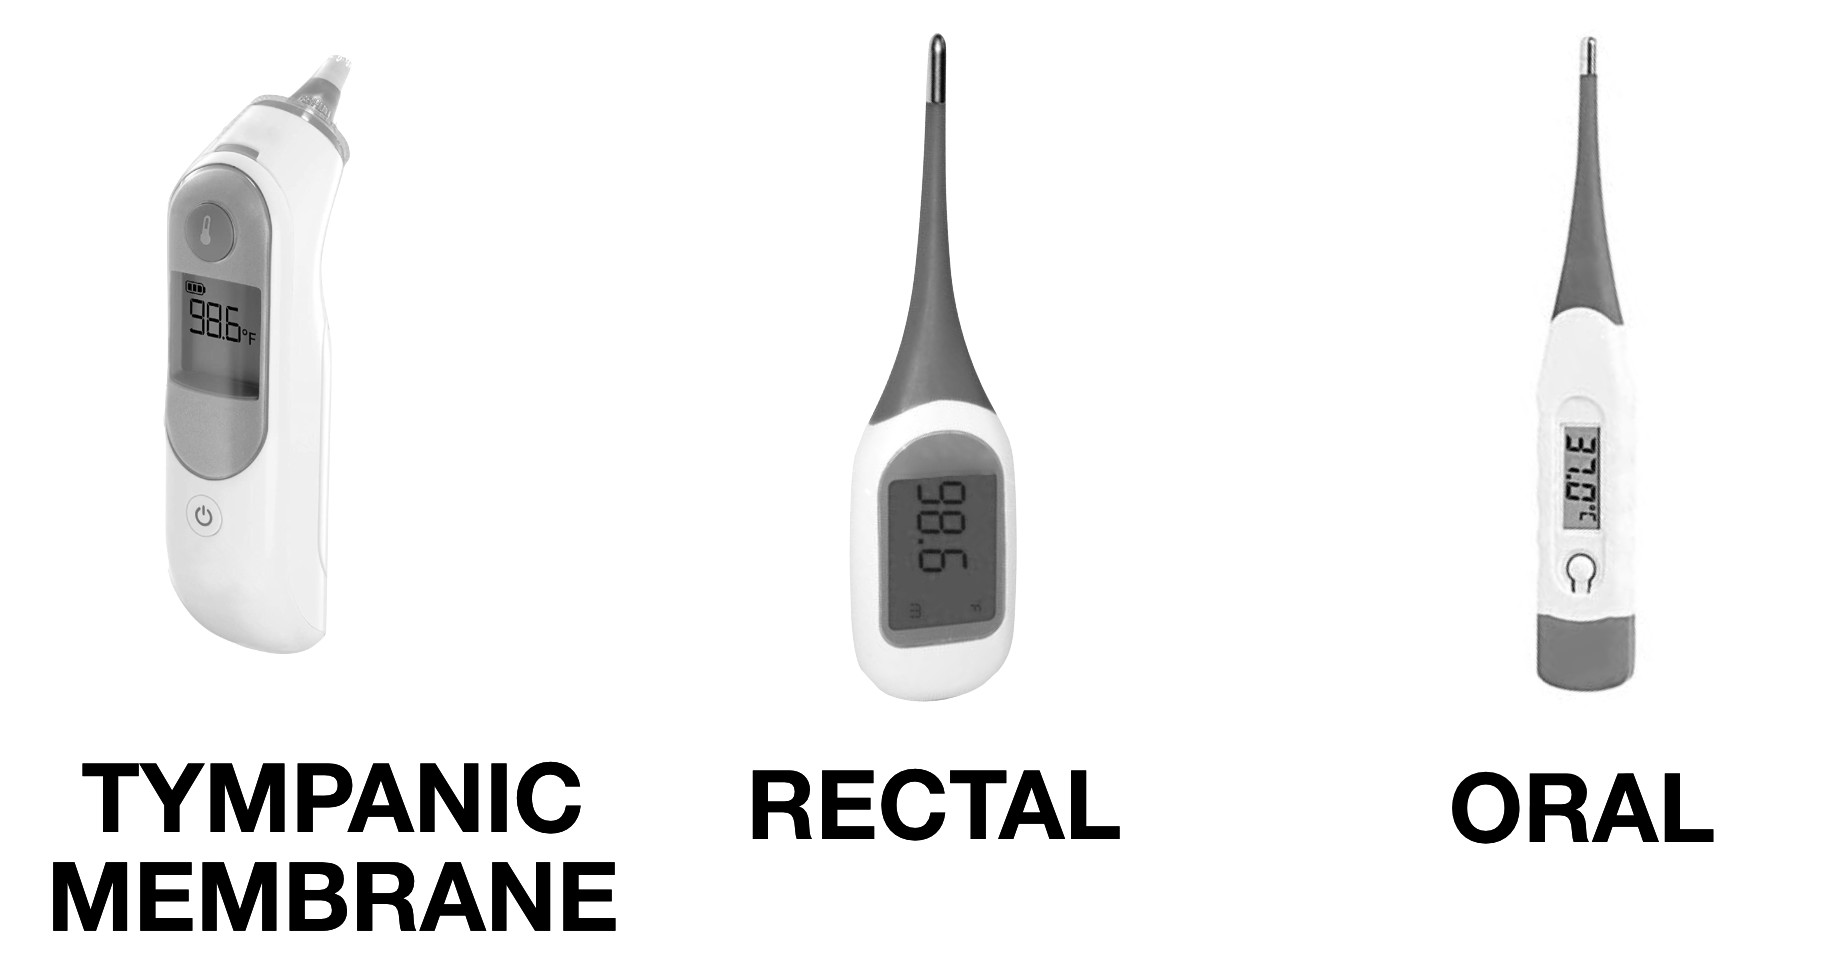
\includegraphics[scale=0.16]{proposal-presentation/images/thermometer_types.jpg}    
    \end{center}
\end{frame}

\begin{frame}{Motivation}
    \begin{center}
        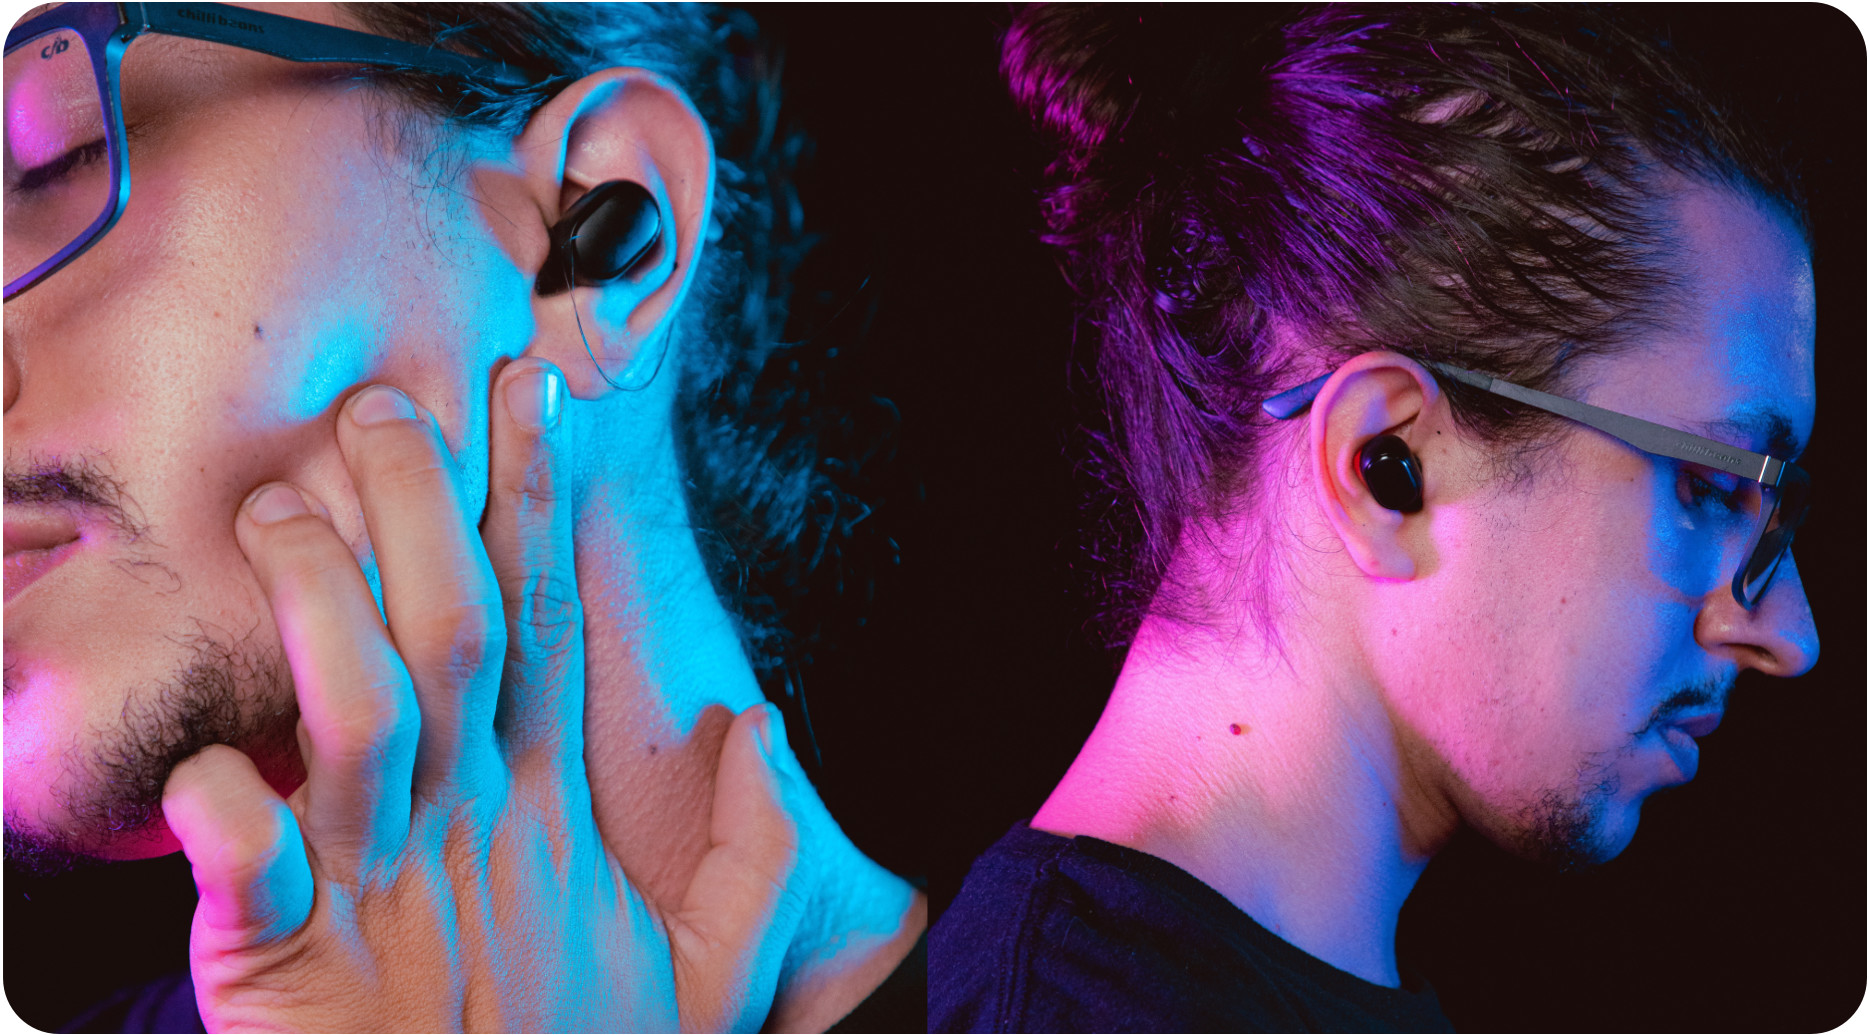
\includegraphics[scale=0.16]{proposal-presentation/images/inears/earbuds_picture.jpg}
    \end{center}
\end{frame}

\section{Problem}
\begin{frame}{Problem}
    \begin{itemize}
        \item accuracy and reliability
        \begin{itemize}
            \item sensor location
            \item skin contact
            \item calibration
        \end{itemize}
        \item tympanic membrane measurement set up
        \begin{itemize}
            \item alignment
            \item ear wax
        \end{itemize}
    \end{itemize}
\end{frame}

\section{Question}
\begin{frame}[fragile]{Question}
    \begin{column}{0.50\textwidth}
        \begin{itemize}
            \item measure temperature at different locations in and around the ears
            \item hypotheses
            \begin{itemize}
                \item correlations with activity
                \item quality can be improved through IMU
                \item combination of signals improves the quality
                \item skin temperature around the ear strongly correlates with core body temperature.
            \end{itemize}
        \end{itemize}
    \end{column}
    \begin{column}{0.45\textwidth}
        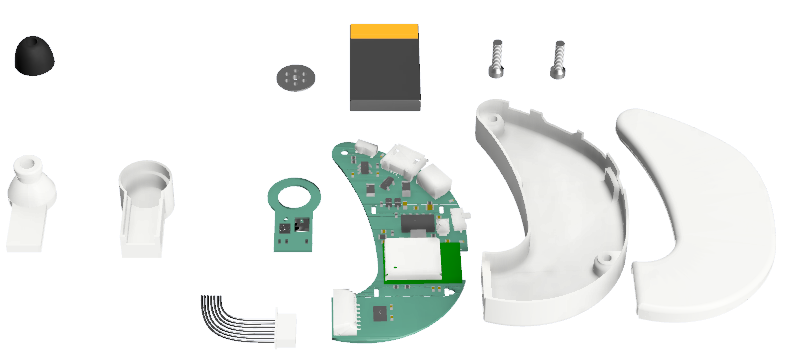
\includegraphics[scale=0.26]{proposal-presentation/images/open_earable_new.png}
    \end{column}
\end{frame}

\begin{frame}[fragile]{Related Work}
\begin{column}{0.47\textwidth}
        \begin{itemize}
        \item huge research field for ...
        \begin{itemize}
            \item temperature measurement on the tympanic membrane
            \item body temperature measurement
        \end{itemize}
        \item no studies on other positions in/around the ear
    \end{itemize}
    \vspace{1cm}
    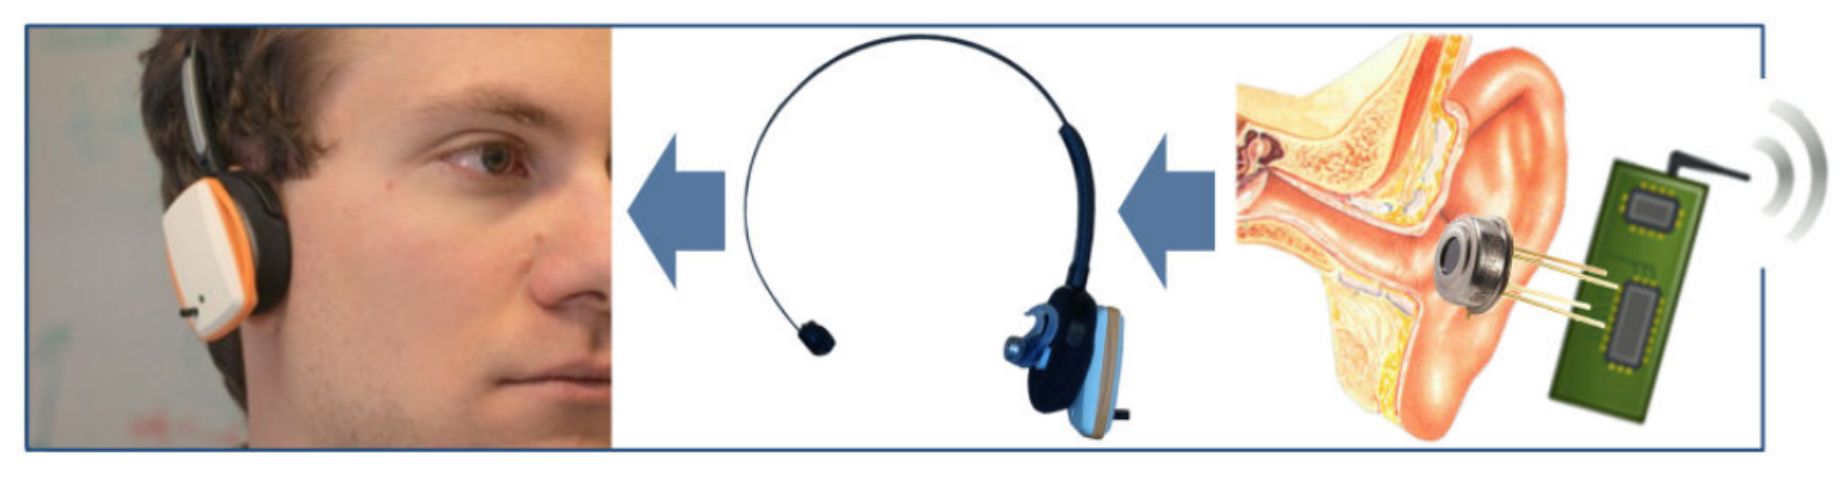
\includegraphics[scale=0.26]{proposal-presentation/images/relatedWork/relatedWork3.png}
    \end{column}
    \begin{column}{0.43\textwidth}
    \vspace{-0.4cm}
        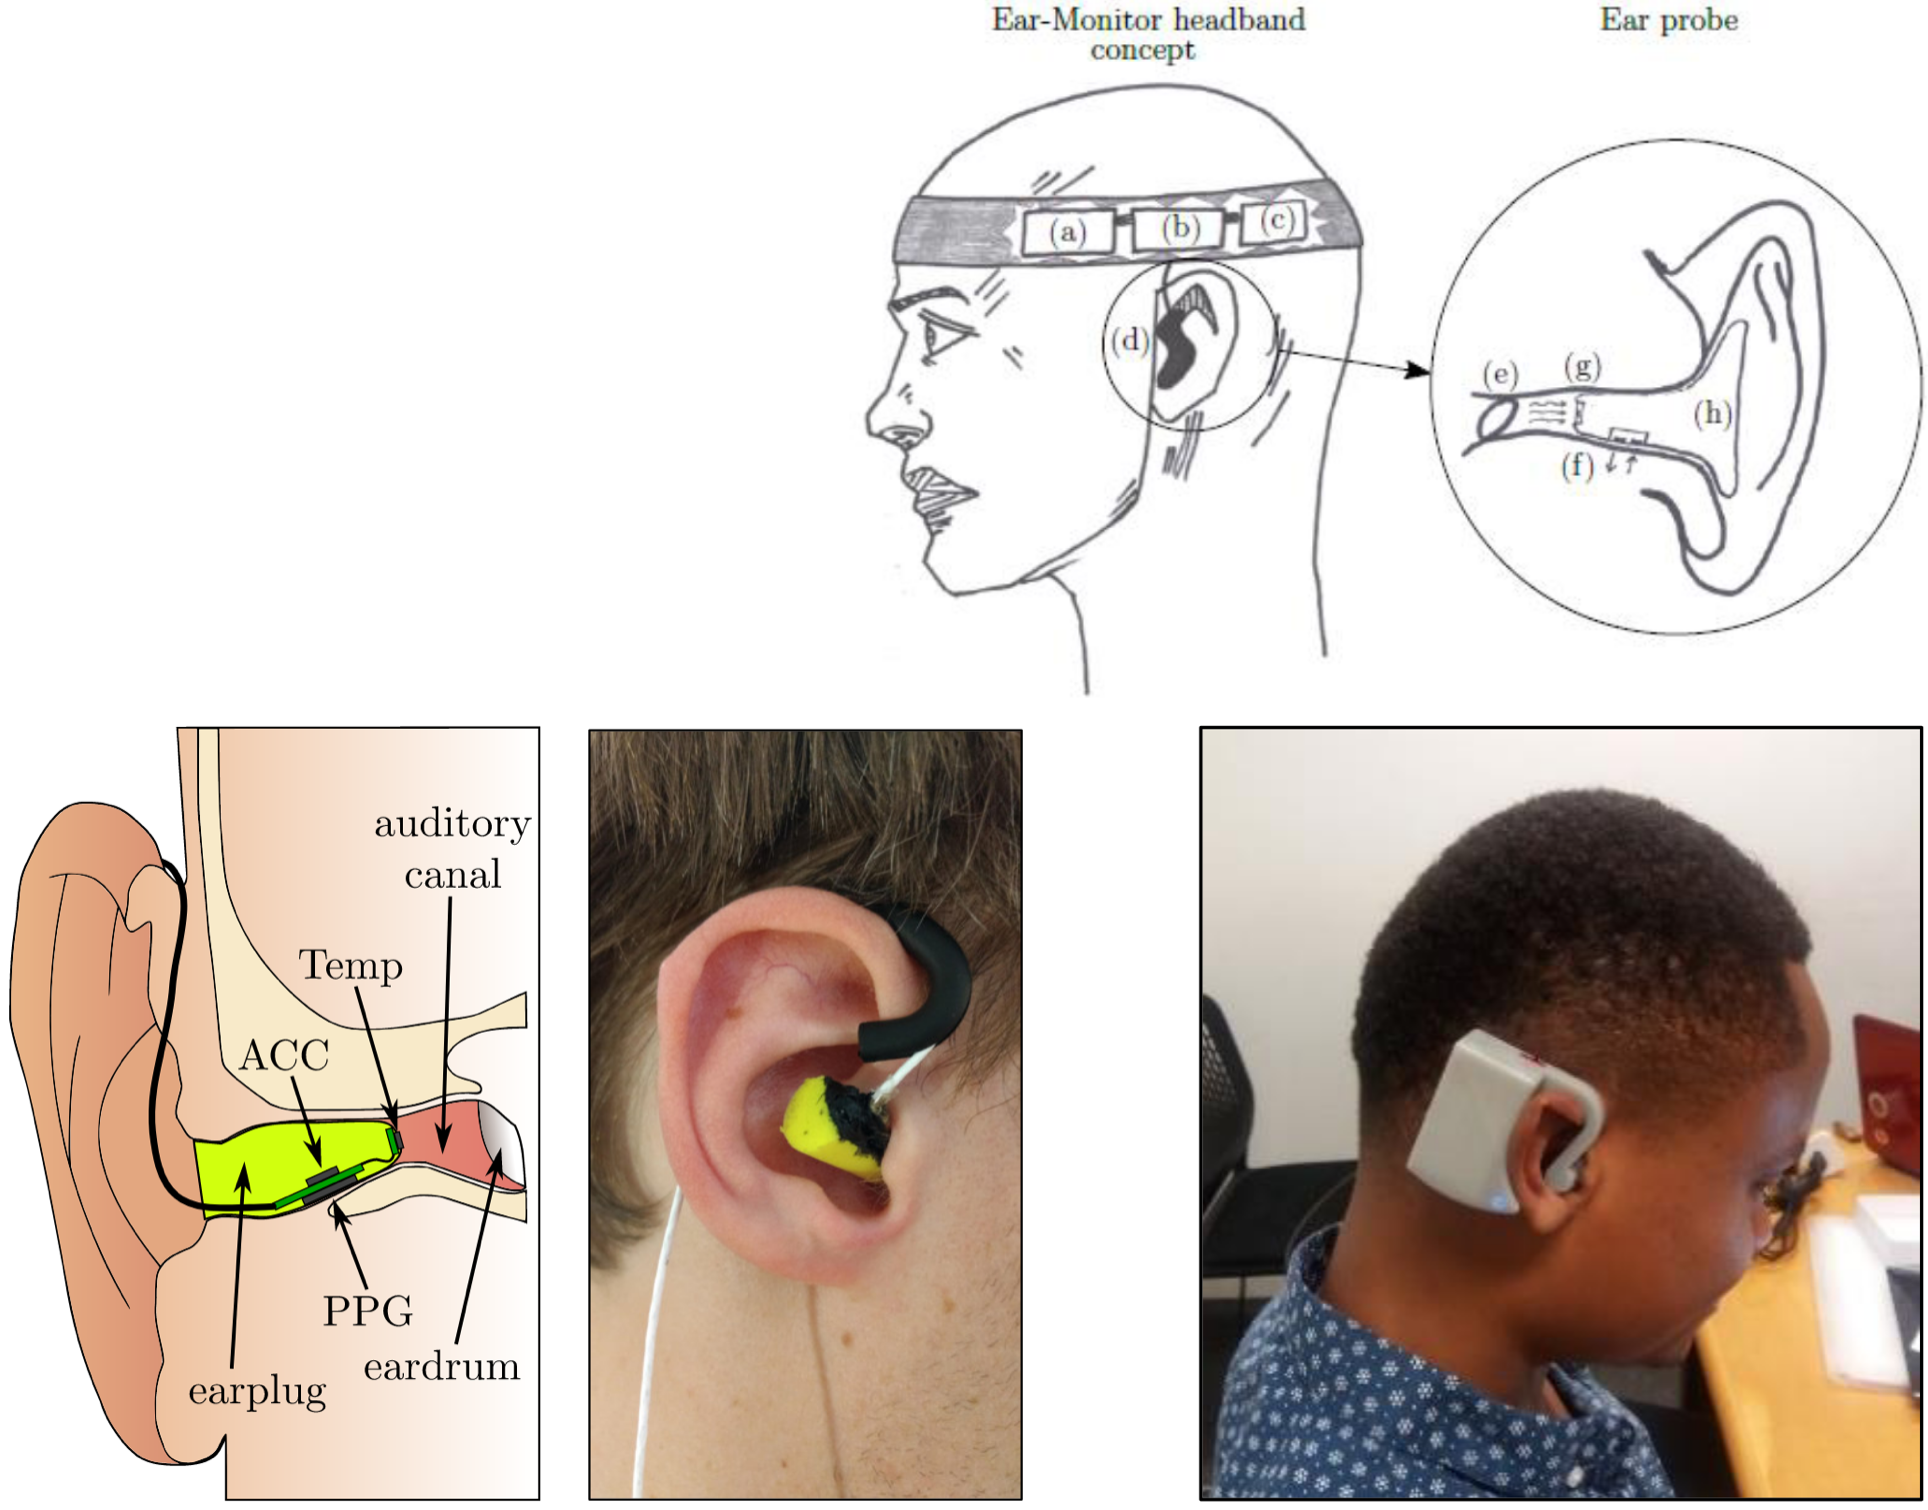
\includegraphics[scale=0.19]{proposal-presentation/images/relatedWork/relatedWorkMerged2.png}
    \end{column}
\end{frame}

\section{Planned Approach}
\begin{frame}{Planned Approach: Phase 1}
    \begin{itemize}
        \item device to measure ear-based temperature data
        \begin{itemize}
            \item OpenEarable platform adaption
            \item MLX temperature sensor
        \end{itemize}
        \item lab study to observe the different positions
    \end{itemize}
    \begin{center}
        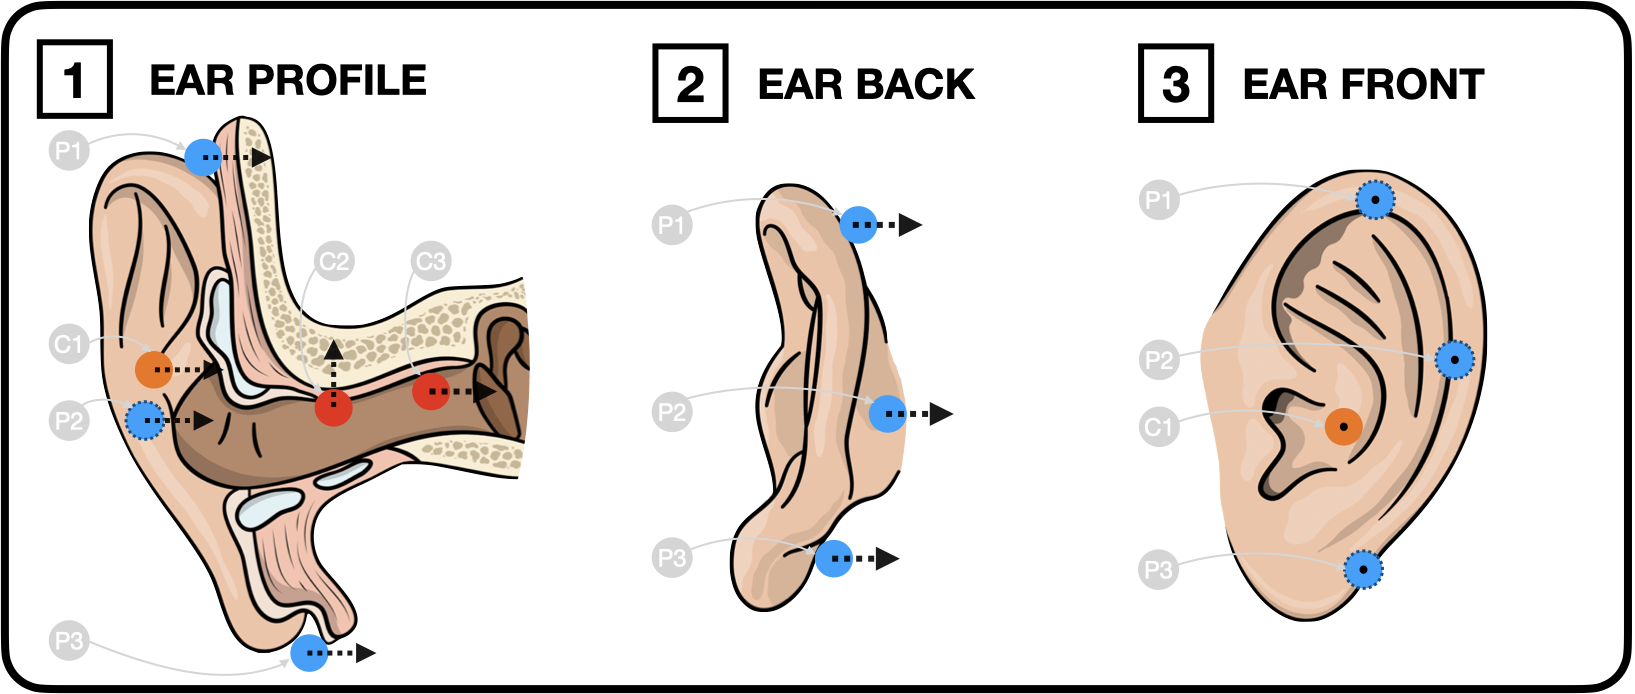
\includegraphics[scale=0.17]{../thesis-doc/images/ear_measurement_points/emp.png}    
    \end{center}
\end{frame}

\begin{frame}{Planned Approach: Phase 2}
    \begin{itemize}
        \item field study during activities
        \begin{itemize}
            \item lying
            \item sitting during work
            \item during multiple workouts
        \end{itemize}
        \item classify temperature-related events of the body
    \end{itemize}
    \begin{center}
        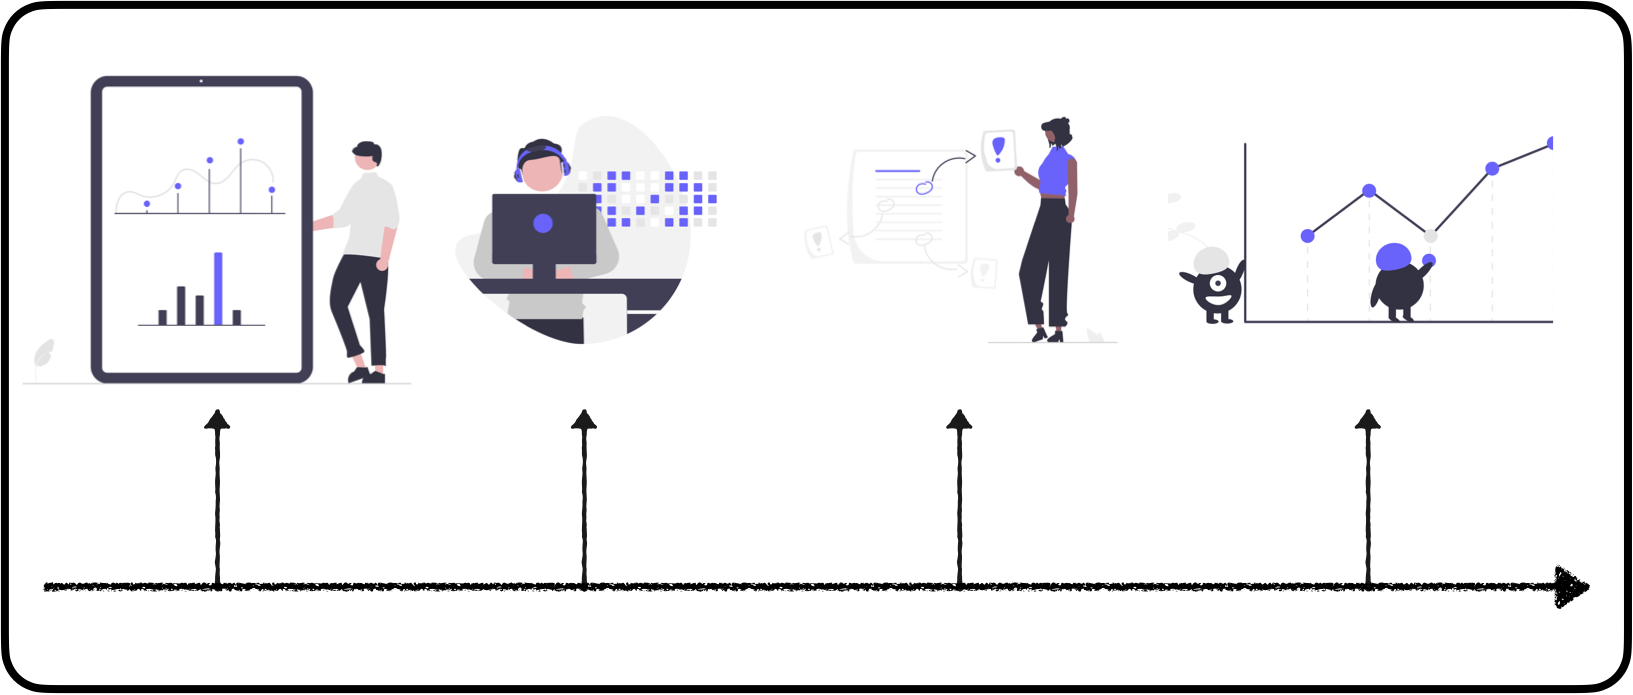
\includegraphics[scale=0.17]{proposal-presentation/images/analytics.png}    
    \end{center}
\end{frame}

\section{Expected Result}
\begin{frame}{Expected Result}
    \begin{itemize}
        \item insights into sensor placement in/around the ear
        \item combination of sensors to improve data quality
        \item support the development of more accurate and reliable wearable devices for biometric applications
    \end{itemize}
\end{frame}

\appendix
\beginbackup

% TODO: Add frames for appendix

% \begin{frame}{Literatur}
% \begin{exampleblock}{Titelbilder Quelle:}
%     asdf    
% \end{exampleblock}
% \end{frame}

\begin{frame}{Literatur}
    \printbibliography
\end{frame}

\section{Farben}
\backupend

\end{document}